%=================================================================
\documentclass[journal,article,submit,electronics,pdftex]{Definitions/mdpi}

%=================================================================
\firstpage{1} 
\makeatletter 
\setcounter{page}{\@firstpage} 
\makeatother
\pubvolume{xx}
\issuenum{1}
\articlenumber{5}
\pubyear{2019}
\copyrightyear{2019}
\newlength\tdima \newlength\tdimb \setlength\tdima{ \fboxsep+\fboxrule} \setlength\tdimb{-\fboxsep+\fboxrule}
\DeclareCaptionFont{white}{\color{white}}
\DeclareCaptionFormat{listing}{
  \parbox{\textwidth}{\colorbox{white}{\parbox{\textwidth}{#1#2#3}}\vskip-3pt}}
\captionsetup[lstlisting]{format=listing,labelfont=white,textfont=white}
\lstset{frame = tlrb, xleftmargin = \tdima, xrightmargin = \tdimb}
\history{Received: date; Accepted: date; Published: date}
\definecolor{aogreen}{rgb}{0.0, 0.5, 1.0}

\newcommand{\norm}[1]{\left\lVert#1\right\rVert}

\usepackage[linesnumbered,ruled,vlined]{algorithm2e}
\newcommand\mycommfont[1]{\ttfamily\textcolor{aogreen}{#1}}
\SetCommentSty{mycommfont}

\SetKwInput{KwInput}{Input}                % Set the Input
\SetKwInput{KwOutput}{Output}              % set the Output

%=================================================================
\Title{Basis pursuit $\ell_1$ minimization and its biomedical applications}

\Author{Lorenzo Simone$^{1}$,\: Sharathchandra Yanamandra $^{2}$}
\AuthorNames{Lorenzo Simone, Sharathchandra Yanamandra}
\address{%
$^{1}$ \quad Università di Pisa (Artificial Intelligence); \; l.simone3@studenti.unipi.it\\
$^{2}$ \quad Università di Pisa (Artificial Intelligence); \; s.yanamandra@studenti.unipi.it}

%\abstract{TODO}

%%%%%%%%%%%%%%%%%%%%%%%%%%%%%%%%%%%%%%%%%%
\begin{document}
\section{Introduction}
\section{Input data and applications}
The objective of providing a dataset or more broadly a specific application for compressive sensing has played a huge role in this project. In literature amongst the major applications in biomedical field such as electroencephalografic (EEG), electrocardiogram (ECG) there is biomedical imaging \cite{donohoCS}.
We provided two applications for basis pursuit:
\begin{itemize}[leftmargin=*,labelsep=5.8mm]
\item reconstructing a signal through a sparse sum of cosines representation
\item ECG signal compression exploiting sparsity in spectral domain
\end{itemize}
\subsection{Sparse sum of cosines}\label{sec:sparse_sines}
The first application covers a sparse sum of cosines reconstruction of an unknown function provided a set of known measurements. Amongst the proposed applications it is the most trivial, but its attractiveness relies on the strong correlation with the foundations of Fourier analysis. The latter is made clear by Fourier theorem stating informally that a periodic function $f(x)$ may be expressed as the sum of a series of sine or cosine terms, each of which with a specific amplitude and phase coefficients, having the name of \textit{Fourier coefficients}. In a detailed definition the problem can be stated as follows:

\begin{equation}
\begin{array}{l}
\text{given a set of ordered pairs also known as observations}\:
\{(x_i, f(x_i))\:|\:i = 1, ... , m\}\\
\text{we proceed solving the following underdetermined linear system of equations} \: (Ay=b) \\
\end{array}
\end{equation}
  
\[
\begin{bmatrix}
a_{11} & a_{12} & \cdots & a_{1n}\\
a_{21} & a_{22} & \cdots & a_{2n}\\
\vdots & \vdots & \ddots & \vdots\\
a_{m1} & a_{m2} & \cdots & a_{mn}
\end{bmatrix}
\begin{bmatrix}
y_1\\y_2\\ \vdots\\y_n
\end{bmatrix}
=\begin{bmatrix}
f(x_1)\\f(x_2)\\ \vdots\\f(x_m)
\end{bmatrix}
\]

\begin{equation}
\begin{array}{l}
A \in \mathbb{R}^{m \times n}\:\text{with}\:m \ll n\:\text{and}\:a_{ij} = cos(jx_i),
y \in \mathbb{R}^n\:\text{having}\:\norm{y}_0 = k \ll n\:\text{and}\:b \in \mathbb{R}^m\\
\text{while minimizing}\: \norm{y}_1\:\text{with each equality constraint summarized as}\:\hat{f}(x_i) = \sum\limits_{j=1}^n  a_{ij} * \cos(jx_i).
\end{array}
\end{equation}

We also investigated known signal waves which can not be expressed as a a discrete sum of cosines, so that we can judge the closeness of our proposed approximation. In order to do so we uniformly distributed sampled points $x_i$ over time domain and retained their respective amplitude values $f(x_i)$ according to the waves:

\begin{itemize}[leftmargin=*,labelsep=5.8mm]
\item Square wave \footnote[1]{For each wave we provide the discrete amplitude function as long as the Fourier series equivalent formulation}: $f(x) = sgn(sin(2\pi fx)) = 
\frac{4}{\pi}\sum\limits_{k=1}^{\infty}{\frac{sin(2\pi(2k - 1)fx)}{2k-1}}$ 
\item Triangle wave: $f(x) = \frac{2a}{\pi}arcsin(sin(2\pi fx)) = 
\frac{8}{\pi^2}\sum\limits_{k=1,3,5,...}^{\infty}{sin(k\pi fx)
\frac{(-1)^{\frac{k-1}{2}}}{k^2}}$
\item Sawtooth wave: $f(x) = -\frac{2a}{\pi}arctan(cot(x\pi f)) = \frac{1}{2}-\frac{1}{\pi}\sum\limits_{k=1}^{\infty}\frac{1}{k}sin(k\pi f x)$
\end{itemize}

The plots over time of the analyzed waves are furtherly depicted in Figure \ref{fig:waves}. 

\begin{figure}[H]
\centering
\subfloat{
  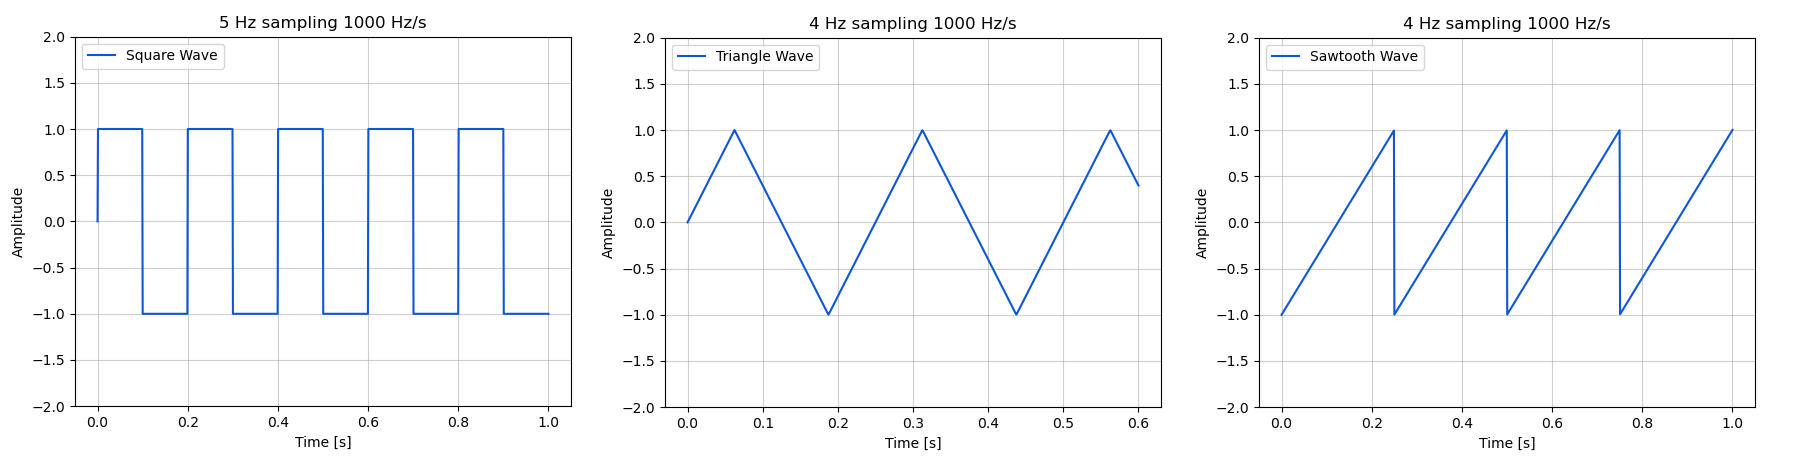
\includegraphics[height=4cm]{Figures/waves.png}
}
\caption{Amplitude plots over time of different signals used to sample observations. Firstly we have the square wave, secondly the triangular and lastly the sawtooth wave.}
\label{fig:waves}
\end{figure}

The sampling procedure allows to construct the $A$ matrix and the $b$ vector used for equality constraints. After solving the linear programming \textit{basis pursuit} problem we can investigate the capability of the sum of cosines reconstruction to approximate the original function used for sampling in Section \ref{results:cosine}.

\begin{figure}[H]
\centering
\hspace*{\fill}
\subfloat[]{%
  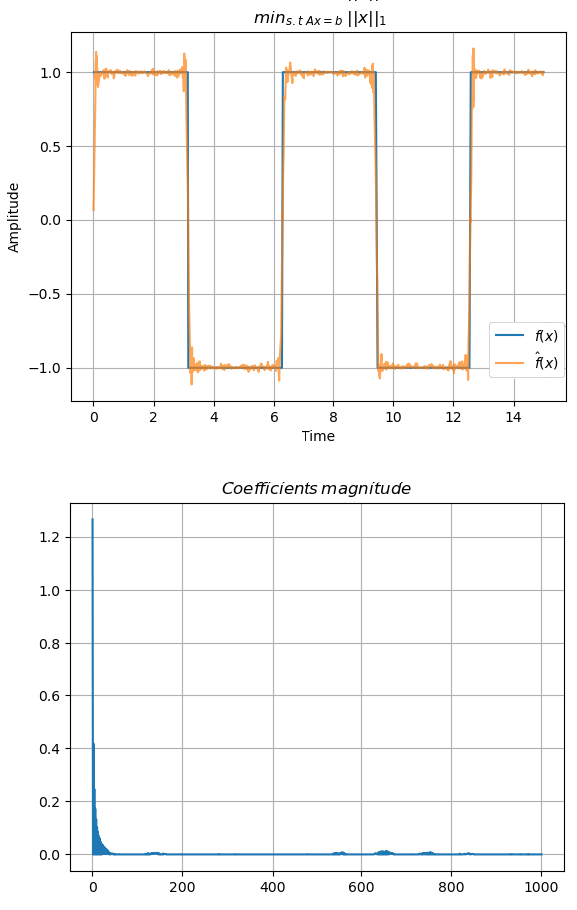
\includegraphics[height=6.5cm]{Figures/squares_fitting.png}
}%
\hspace*{\fill}
\subfloat[]{%
  \includegraphics[height=6.5cm]{Figures/triangle_fitting.png}
}%
\hfill{
\subfloat[]{%
  \includegraphics[height=6.5cm]{Figures/sawtooth_fitting.png}%
}}
\hspace*{\fill}
\caption{The first row depicts the overlapping of the original signal in blue $f(x)$ used for sampling and the reconstructed sum of cosines approximation $\hat{f}(x)$. The sparsity of the solution coefficients can be visualized by the second row of plots. (\textbf{a}) Square wave, (\textbf{b}) Triangle wave, (\textbf{c}) Sawtooth wave, }
\label{fig:fitting}
\end{figure}

\subsection{ECG signal compression}\label{sec:ecg_signal}
In this application we utilize ECG signals by undersampling the original signal given a percentage of compression and reconstructing it by using compressed sensing. The validity of compressed sensing in this application is based on the fact that the signal in the frequency domain is highly sparse. Amongst all the configurations, we are interested in the simplest and most sparse solution according to the $\ell_1$-norm matching exactly or as closely as possible the known data.\\
In Figure \ref{fig:ecg_dft} we show  on the left a sample of an ECG signal sampled at 1kHz for 5 seconds with its Discrete Cosine Transform (DCT), we preferred using the latter over Discrete Fourier Transform (DFT) becausing having to deal with real sparse coefficients was more efficient than having complex ones.

\begin{figure}[H]
\centering
\subfloat{
  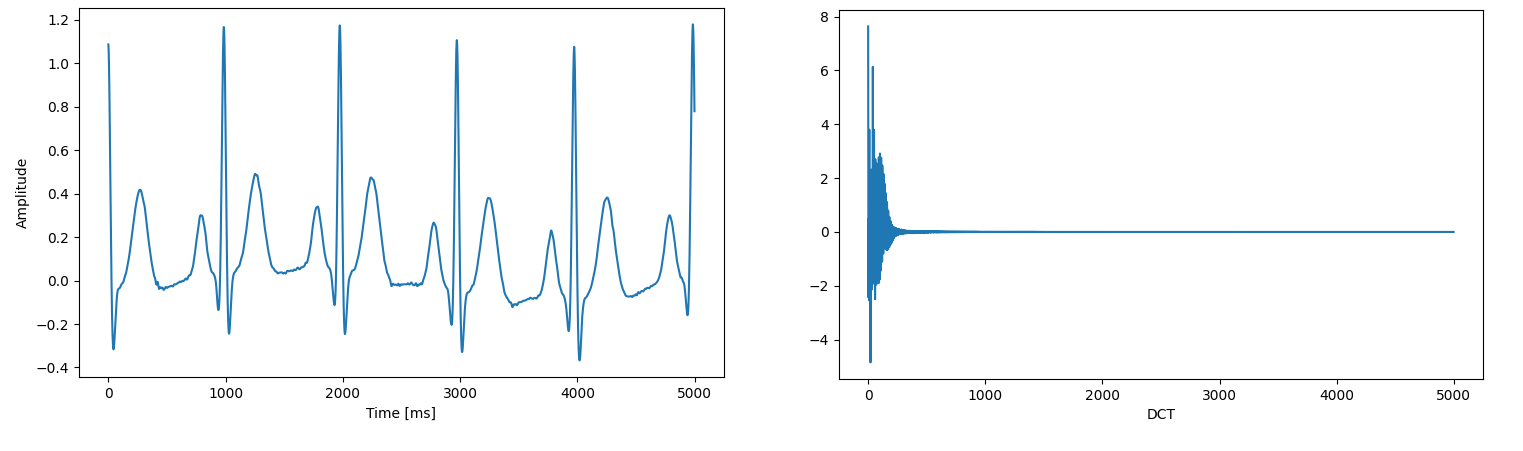
\includegraphics[height=5cm]{Figures/ecg_dct.png}
}
\caption{\textbf{(a)} ECG signal sampled at 1kHz for 5 seconds having an average of 60 beats per minute, \textbf{(b)} Discrete cosine transform of the input ECG signal representing a highly sparse basis.}
\label{fig:ecg_dft}
\end{figure}

As a recap we are still solving the task:
\begin{equation}
\min\limits_{x\:s.t.\:Ax = b}\norm{x}_1
\end{equation}

Specifically, in the context of this application the vector $b$ contains the data samples in the temporal domain and the solution $x$ belongs to the frequency domain, the role of the short fat matrix $A \in \mathbb{R}^{m \times n}$ is to perform both sampling and transformation from frequency to temporal domain.\\
In order to construct the matrix A we followed a well established methodology \cite{matrixA,candes}. In our application the ECG signal can be regarded as a vector $f$ being a linear combination of the DCT expressed as $\psi$.
\begin{equation}
f = \psi c
\end{equation}
The sampling procedure consists in a linear operator $\phi$
\begin{equation}
b = \phi f
\end{equation}
From the abov\times 10^{mentioned equations it follows that $A = \phi \psi$, and it is made of the rows sampled from the domain transform matrix $\psi$, being the Inverse Discrete Cosine Trasnform (IDCT) applied to the columns of the identity matrix.
A visual representation of the matrix $A$ applied to this task is depicted in Figure \ref{fig:amatrix}, having dimensions $1000 \times 5000$, being respectively the sampling rate (1kHz) and the elapsed time (5000 ms).
\begin{figure}[H]
\centering
\subfloat{
  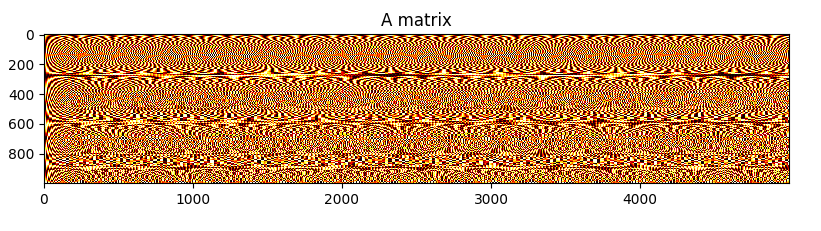
\includegraphics[height=4cm]{Figures/AMatrix.png}
}
\caption{Visual representation of the matrix $A$ applied to the ECG signal wave depicted in Figure \ref{fig:ecg_dft}, having dimensions $1000 \times 5000$, being respectively the sampling rate (1kHz) and the elapsed time (5000 ms)}
\label{fig:amatrix}
\end{figure}

Once the building blocks of the original problem are constructed we solved it and converted the solution from the frequency to the temporal domain. We have investigated different percentages of compression rate, which is involved in the random sampling process, obtaining satisfying results even with only 10\% of the original signal data.\\ We provide an example of the overall process: starting from the ECG signal depicted in Figure \ref{fig:ecg_dft} we uniformly random sampled 10\% of it and we constructed the A matrix, obtaining the solution to the classical basis pursuit problem which was finally transformed in the temporal domain. The second row from Figure \ref{fig:reconstruction}, qualitatively describes the result of the reconstruction using the above described process and settings for the compression rate.

\begin{figure}[H]
\centering
\subfloat{
  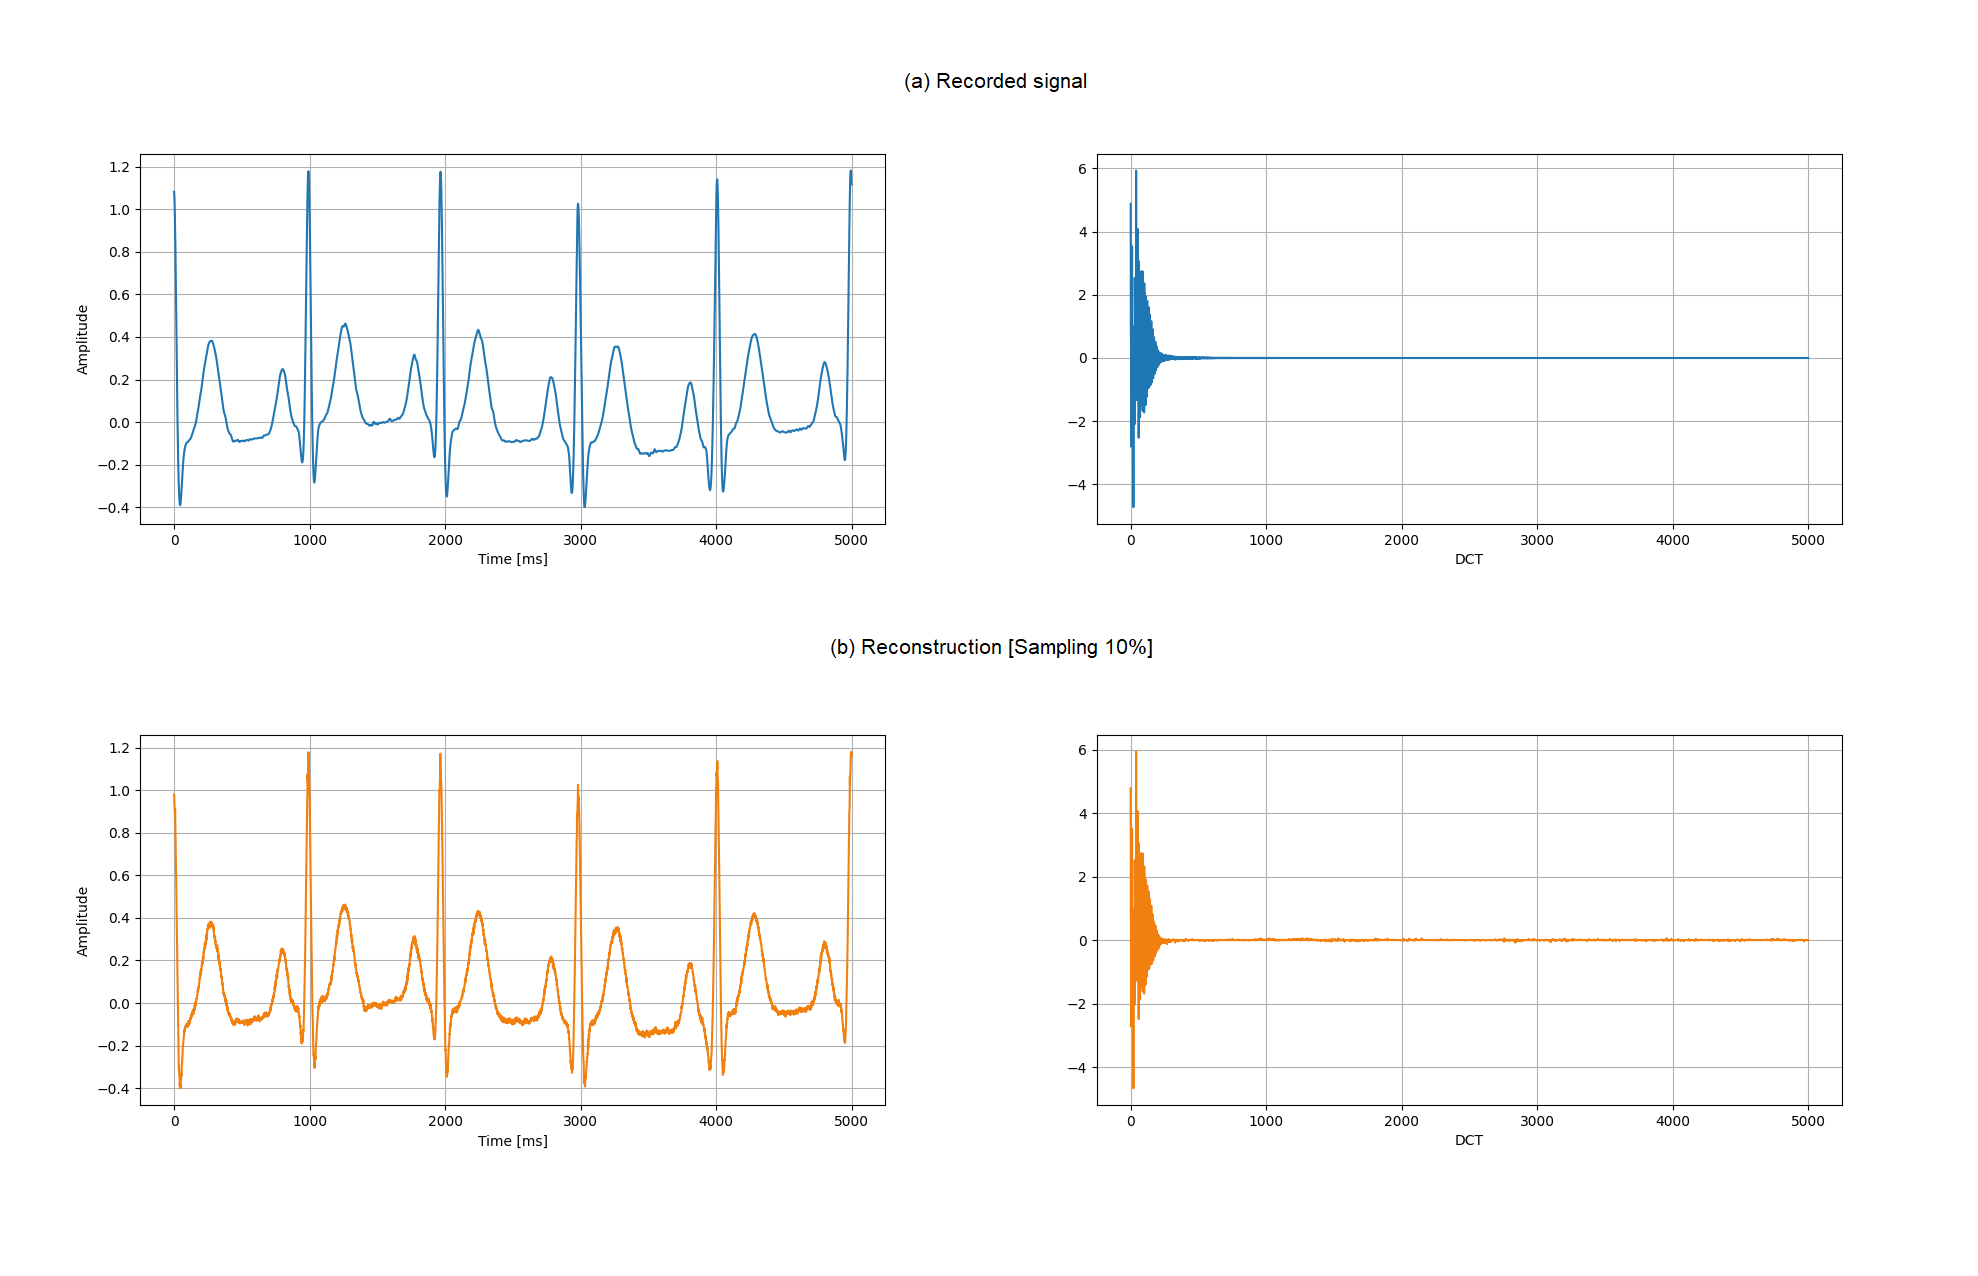
\includegraphics[height=11cm]{Figures/reconstruction.png}
}
\caption{\textbf{(a)} Original ECG signal sampled at 1kHz for 5 seconds having an average of 60 beats per minute next to its DCT, \textbf{(b)} Reconstructed ECG signal from random sampling only 10\% of the original wave next to its DCT representing the solution.}
\label{fig:reconstruction}
\end{figure}


\section{Basis Pursuit as Linear Programming}

The original Basis Pursuit (BP) is a convex optimization problem formulated as:
\begin{equation}
\label{eqn:BP}
\min\limits_{x\:s.t.\:Ax = b}\norm{x}_2,
\end{equation}
the assumption of convexity for this problem holds from the two basic properties for the set on which we optimize $\mathbb{R}^n$ and for the objective function:

\begin{enumerate}
  \item \textbf{Convex set:}\\
  Any convex combination of two vectors in $\mathbb{R}^n$, does still belong in $\mathbb{R}^n$.\\\\
  Let x,y $\in \mathbb{R}^n$ and $\alpha \in [0,1]$\\
  $\alpha x + (1- \alpha)y = \langle \alpha x_k : k \in \mathbb{N} \rangle$ +
  $\langle (1-\alpha) y_k : k \in \mathbb{N} \rangle$ = $\langle \alpha x_k + (1-\alpha) y_k : k \in \mathbb{N} \rangle = z \in \mathbb{R}^n$ \\
  \item \textbf{Convex objective function}\\
  From basic properties of every $p-$norm and using triangle inequality we can verify that our objective function $\norm{x}_1$ is convex:\\\\
$f: V\xrightarrow[]{} \mathbb{R} \: \text{is convex} \Leftrightarrow \forall v,w \in V, \lambda \in [0,1] : f(\lambda v + (1-\lambda)w) \leq \lambda f(v) + (1-\lambda)f(w),$ 
which applied to $\ell_1$ and norms in general gets straightforwardly: \\\\
$\norm{\lambda v + (1-\lambda)w}_1 \leq \norm{\lambda v}_1 + \norm{(1-\lambda)w}_1 = \lambda\norm{v}_1 + (1-\lambda)\norm{w}_1 $.
\\
\end{enumerate}
\subsection{LP equivalent formulation}

We proceed by reformulating the original problem as a linear programming problem having an equivalent form and a well-defined constant gradient $\nabla f(v) = \boldsymbol{1}^{2n}$: \\
\begin{equation}
x = v^+ - v^-,\:\:\:v_i^+ = \max{\{x_i, 0\}},\:\:\: v_i^- = \max{\{-x_i, 0\}}
\end{equation}
Then Basis Pursuit (\ref{eqn:BP}) can be also written like:\\
\begin{equation} \label{eq:reformulation}
\begin{array}{l}
\min\limits_{v}\sum_{i=1}^n{v^+_i + v^-_i}\\\\
\text{subject to}\: A(v^+ - v^-) = b,\\
v^+ \succeq \mathbf{0}\\
v^- \succeq \mathbf{0}
\end{array}
\end{equation}

\subsection{Asymmetric dual pair formulation}

Usually, in order to find an optimal value for the objective function for an LP we make reference to the dual of the asymmetric pair, being another LP problem having many syntactical and non properties in common with the first. We proceed by defining the three main concepts behind our \emph{revised simplex} implementation, in order to solve the \emph{basis pursuit}.

First of all we define the primal (P) and the dual (D) from the standard asymmetric pair formulation:
\begin{equation}
(P) \hspace{10pt}\max \{cx : Ax \leq b\} \hspace{60pt}(D)\hspace{10pt}
\min \{yb : yA = c, y \geq 0 \}
\end{equation}

We also provide the new matrix $A' \in \mathbb{R}^{m \times 2n}$ and the solution vector $v \in \mathbb{R}^{2n}$ based on the reformulation from (\ref{eq:reformulation}), this requires a change of sign for the respective columns.

\begin{equation} \label{eq:partitioned_system}
A' = 
    \begin{bmatrix}
    A & -A\\
    \end{bmatrix}
    \hspace{30pt}
    v =
    \begin{bmatrix}
    v^+\\v_{-}
    \end{bmatrix}
    \hspace{30pt}
\end{equation}

\begin{equation*}
\begin{array}{llllclll}
& \text{max}         & b_1 x_1  & + b_2 x_2   & {}+{\dots}+{} & b_m x_m  \\
& \text{subject to } & A_{11}^Tx_1 & + A_{12}^Tx_2 & {}+{\dots}+{} & A_{1m}^Tx_m \leq c_1\\
(P)\hspace{20pt}&             &             &               &\vdots         &\\
& & A_{2n,1}^Tx_1 & + A_{2n,2}^Tx_2 & {}+{\dots}+{} & A_{2n,m}^Tx_m \leq c_{2n}\\
\\\\\\
& \text{min}         & c_1 v_1^+  & + c_2 v_2^+   & {}+{\dots}+{} & c_{2n} v_{n}^-  \\
& \text{subject to } & A_{11}v_1^+ & + A_{12}v_2^+ & {}+{\dots}-{} & A_{1,2n-1}v_{n-1}^- & - A_{1,2n}v_n^- & {} = b_1 \\
(D)\hspace{20pt}&             &             &               &\vdots         &                    &             &          \\
 &  & A_{m,1}v_1^+ & + A_{m,2}v_2^+ & {}+{\dots}-{} & A_{m, 2n-1}v_{n-1}^- & -A_{m, 2n}v_{n}^- & {} = b_{m} \\
 &  & v_1^+,  & v_2^+,  & {}\:{\dots}\:{}  & v_{n-1}^-,  & v_{n}^-,  & \:\:\geq{0}  \\
\end{array}
\end{equation*}

We can notice from both the above formulations, that neither the primal (P) nor the dual (D) exhibit an admissible basis for starting the implementation of the \emph{revised dual simplex} algorithm. Our objective from this phase is retrieving an admissible starting basis B, being a projection vector exploiting the sparsity of the A matrix and its resulting nonsingular submatrix $A_B$.

We proceed by establishing a working method for finding a starting basis $B$ applied to our applications described in Section \ref{sec:ecg_signal} and Section \ref{sec:sparse_sines}, relying on a foundamental theorem stating that the dual of the dual is the primal and by applying the two-phase method, also usually known as Big-M method \cite{bigMmethod}. An example of the latter applied to our problem is described in eq. \ref{eq:auxiliary}. 

\begin{equation}
\begin{array}{llllcllllll}\label{eq:auxiliary}
& \text{max}         & b_1 x_1  & + b_2 x_2   & {}+{\dots}+{} & b_m x_m  \\
& \text{subject to } & A_{11}^Tx_1 & + A_{12}^Tx_2 & {}+{\dots}+{} & A_{1m}^Tx_m & \leq c_1\\
(P')\hspace{20pt}&             &             &               &\vdots         &\\
& & A_{2n,1}^Tx_1 & + A_{2n,2}^Tx_2 & {}+{\dots}+{} & A_{2n,m}^Tx_m & \leq c_{2n}\\\\
& & x_1  \hspace{15pt}{}{\dots}{} &  0 &  \leq M &  & \\
 &            &   \vdots  \hspace{20pt}\ddots         &               &         &\\
& & 0 & +x_m  & \leq M &  & \\
\\\\\\
& \text{min} & c_1 v_1^+  & + c_2 v_2^+   & {}+{\dots}+{} & c_{2n} v_{n}^- 
& + M w_{1} & {}+{\dots}+{} & M w_m \\
& \text{subject to } & A_{11}v_1^+ & + A_{12}v_2^+ & {}+{\dots}-{}  &  A_{1,2n}v_n^- & w_1 & +0 & {} = b_1 \\
(D')\hspace{20pt}&             &             &               &\vdots         &                    &       \vdots  \hspace{20pt} \ddots     &         \\
 &  & A_{m,1}v_1^+ & + A_{m,2}v_2^+ & {}+{\dots}-{} & A_{m, 2n}v_{n}^-  & 0 & w_m & {} = b_{m} \\
 &  & v_1^+,   & {}\:{\dots}\:{}  & v_{n-1}^-,  & w_{1}, & {}\:{\dots}\:{} & w_{m} & \:\:\geq{0}  \\
 
\end{array}
\end{equation}

By choosing M as a vector having positive and sufficiently big components, (D') is actually equivalent to the formulation of (D), the original dual. In detail, since the dual is bounded below, also the auxiliary form of the dual will share the same property \cite{ricercaoperativa}. 

The starting point of the algorithm is now represented by the artificial basis $B = \{2n+1, ..., 2n + 1 + m\}$, building the matrix $A_B = I$ and having an admissible starting solution for the dual. 

\subsection{Linear algebra: Forrest-Tomlin update}
We have to solve linear systems involving the square matrix $A_B$ for each iteration, but we 
never calculate the inverse basis matrix explicitly just to solve these systems. 
Instead, we maintain an LU factorization for 30 iterations, by using triangular substitutions to recover the intermediate solutions. 

These assumptions are based on the fact that it would be expensive to recompute the LU factorization at each step, since $A_B$ is changing only by a single row between iterations. Actually, we could have even used a pivoting strategy based on the assumption that for some applications of BP, the A matrix is usually sparse and having specific symmetric properties, but this is left as a further optimization \cite{num_optimization}.

For instance starting from an LU factorization of $A_B$, with rows and columns already permuted:

\begin{equation} \label{eq:LU}
LU = A_B    
\end{equation}

the system $A_B \bar{x} = b_B$ can be solved by the following two-steps easier procedures:
\begin{equation}
L\lambda = A_B , \hspace{20pt} U \bar{x} = \lambda,
\end{equation}
similarly all the systems in the form $yA=c$ are solved in the same manner, just considering that they can be rearranged in $A^Ty^T = c^T$. 

Straightaway, we discuss the procedure for updating the triangular matrices L and U at each step, excluding the ones in which we refactor the full LU (first iteration and multiples of 30). As we have already stated above, the only change in the matrix $A_B$ is the row $A_k$ substituting $A_h$ in the basis since $h\in B$ and $k\in N$. From now on we will refer to this operation as a column update, since it would be the same by considering $A_B^T$ instead of $A_B$. We will refer to the updated matrix as $A_B^+$. 

Now, by rewriting (\ref{eq:LU}) we end up with $U = L^{-1}A_B$ and $L^{-1}A_B^+$ is still an upper triangular matrix except in column h, which was changed (\ref{fig:update}.a). With the objective of moving the non-upper triangular part of the matrix to the last row, we can apply cyclic permutations shifting column h to the last column (\ref{fig:update}.b). The latter is straightforward, since we can start from the original vector of the columns of $A_B^+$ being $c = [1,2,...,h,..,n]$ and compute the permutation vector as $\pi = [1,2,...,n-h+2,...,n,h]$ which applied to the identity matrix will get $P_1$, the row-shifting matrix and $P_1^T$ the related column-shifting one. We propose a graphical representation of this update process in Figure \ref{fig:update}, by using the MATLAB \emph{spy} utility plotting function for non-zero patterns in a matrix applied to one of our iterations of the running proposed algorithm.

\begin{figure}[H]
\centering
\subfloat{
  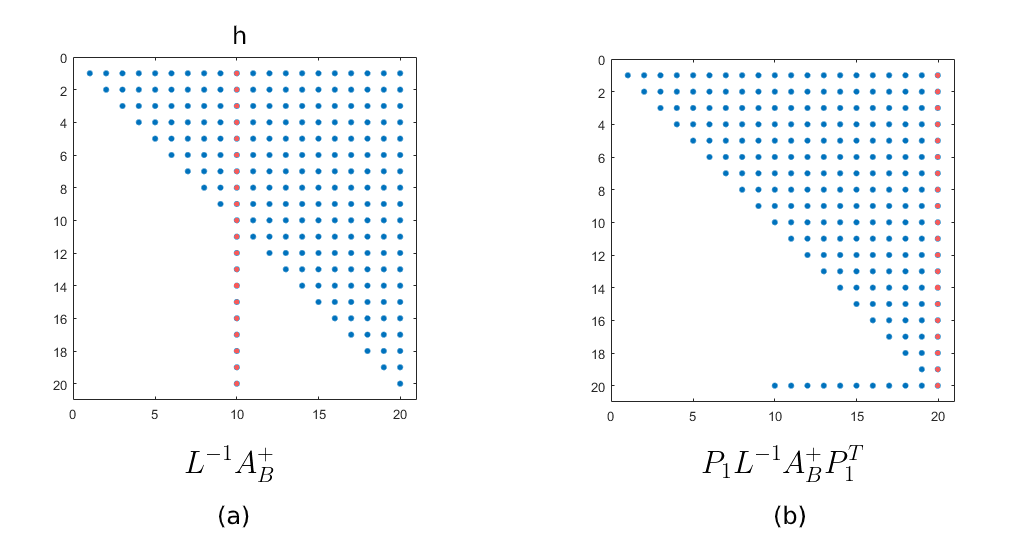
\includegraphics[height=6cm]{Figures/update.png}
}
\caption{\textbf{(a)} The index for the updated column in the matrix $A_B^+$ is \emph{h}, resulting in a pattern having a single column away from an upper triangular form. \textbf{(b)} After applying the permutation for both rows and columns respectively multiplying by $P_1$ and $P_1^T$, we end up in a situation in which only the last row is full of non-zeros.}
\label{fig:update}
\end{figure}

From the matrix $P_1 L^{-1} A_B^+ P_1^T$ we can retrieve $P_1 L^{-1} A_B^+ P_1^T = L_1 U_1$ by sparse Gaussian eliminations, where $L_1$ is different from the identity only in the last row and also $U_1$ is identical to $P_1 L^{-1} A_B^+ P_1^T$ except for the last row. Finally we can calculate the updated factorization for $A_B$ as:
\begin{equation}
    A_B^+ = L^+ U^+, \hspace{20pt} \text{where} \hspace{10pt} L^+ = LP_1^TL_1 \hspace{10pt} \text{and}  \hspace{10pt} U^+ = U_1P_1
\end{equation}

\subsection{Proposed algorithm pseudocode}

\begin{algorithm}[h]
\DontPrintSemicolon
  
  \KwInput{
  \textbf{A} coefficient matrix\\
  \hspace{32.5pt}\textbf{b} vector\\
  \hspace{32.5pt}\textbf{c} cost vector\\
  \hspace{31.5pt}\textbf{B} admissible basis\\
  \hspace{31.5pt}\textbf{maxIter} allowed maximum iterations\\
  \hspace{31.5pt}\textbf{tol\_set} primal empty set tolerance\\
  \hspace{31.5pt}\textbf{tol\_opt} optimal solution tolerance\\
  \hspace{31.5pt}\textbf{verb} verbose mode flag\\
 
  }
  \KwOutput{ $\boldsymbol{\bar{x}}$ \hspace{0.5pt} vector\\
  
  \hspace{38.5pt} $\boldsymbol{\bar{y}}$ \hspace{0.5pt} vector\\\\
  \hspace{38.5pt} \textbf{cost\_vector} \hspace{0.5pt} objective function value over iterations\\\\}
  \vspace{20pt}
  j = 1;\\
  \vspace{5pt}
  refactor = 30;\\
  \vspace{5pt}
  \While{j < maxIter}
   {
        \tcp*{Perform LU for the first time on $A_B$ or after \#\emph{refactor} iterations}
   		\If{ j \% refactor == 0}
    {
        [L, U] = lu($A_B$);\\
        
    }
    \Else{
        \tcp*{Forrest-Tomlin update of LU factorization}
        \pi_1 = [1,...,n-2,n-1,h]\\
        \vspace{5pt}
        P_1 = I([\pi_1],:);\\
        \vspace{5pt}
        [L_1, U_1] = lu(P_1L^{-1}BP_1^T);\\
        \vspace{5pt}
        L = LP_1^TL_1;\\
        \vspace{5pt}
        U = U_1P_1;\\
        \vspace{5pt}
    }
    
    \tcp*{Solving $x = A_b^{-1} b_b$ by LU factorization}
    d = solve(L,b_b);\\
    \vspace{5pt}
    $\bar{x}$ = solve(U,d);\\
    \vspace{5pt}
     \tcp*{Solving $\bar{y_B} = cA_b^{-1}$ by LU factorization}
    $\bar{y}$ = [0,0,...,0]^m;\\
    \vspace{5pt}
    $\lambda$ = solve(L,c^T);\\
    \vspace{5pt}
    $\bar{y_B}$ = solve(U,$\lambda$);\\
    \vspace{5pt}
    \tcp*{Optimal solution check}
    \If{$A_N \bar{x} + \text{tol\_opt} \le b_N$}
    {
        \Return \: 'Optimal solution found'
    }
    
    
    \vspace{5pt}
    v = solve(L,A_k^T);\\
    \vspace{5pt}
    \eta_B = solve(U,v);\\
    
    \tcp*{Primal set emptiness check}
    \If{\eta_B \le  \text{tol\_set}}
    {
        \Return \: 'Primal set is empty'
    }
    \tcp*{Bland's anticycle rule}
    k = N(find(A_nx > b_N, 1,\:'first'));\\
    h = B(find(y/\eta \:and\: \eta > 0, 1,\:'first'));\\
    \vspace{5pt}
    \tcp*{Basis update}
    B(B==h) = k;\\
    \vspace{5pt}
    N(N==k) = h; \\
    \vspace{5pt}
    j++;
   }
\caption{\emph{Revised dual simplex (Forrest-Tomlin update, Bland's anticycle rule)}}
\end{algorithm}

\clearpage
\section{Experimental results}

\subsection{Sum of Cosines reconstruction}
\label{results:cosine}

The first application covers a sparse sum of cosines reconstruction of unknown functions provided a set of known measurements. As a preliminary step, we tested the algorithm for functions which could be perfectly reconstructed, in detail, we used the following functions for generating the points:

\begin{itemize}
  \item $f(x) = \cos(5x) + \cos(100x)$
  \item $f(x) = \cos(5x)$
\end{itemize}

Throughout each of the applications covered in this section we managed the tricky problem of tuning tolerances and stopping conditions for the method. The algorithm includes two stopping conditions referring respectively to the primal set being empty and to an optimality check. We experienced different values ranging from $10^{-8}$ to $10^{-5}$ not noticing a substancial difference in the outcome. Finally, we stuck to the value of the primal empty set check being to $10^{-6}$ and $10^{-7}$ for optimal condition. 


In order to test and measure the accuracy of the reconstruction compared to the original signal, we have used the Mean Squared Error (MSE) and the Pearson correlation coefficient ($\rho$), defined as:

\begin{equation}
    MSE(A,B) = \frac{1}{n}\sum_{i=1}^n{(A_i - B_i)^2} \hspace{30pt}
    \rho(A,B) = \frac{1}{n-1}\sum_{i=1}^n{(\frac{A_i - \mu_A}{\sigma_A})}{(\frac{B_i - \mu_B}{\sigma_B})}
\end{equation}

We ran the algorithm testing it with various combinations of the number of variables (n) and number of observations (m).
For these specific trivial instances, the exact solution is perfectly recovered in few iterations, obtaining an error smaller than the machine epsilon. Based on the latter, we simply report the best results obtained with a single combination of parameters in Table \ref{table:cos_results}.

\begin{table}[htb]
    \centering
    \begin{tabular}{lcccccc}
        \toprule
        $f(x)$ & n & m & $\norm{Ax-b}_2$ & $\norm{x}_1$ & MSE & $\rho$ \\
        \midrule
        $\cos(5x) + \cos(100x)$ & 500 & 100 & $2.246437 \times 10^{-15}$ & 2 & $5.643129\times 10^{-32}$ & 1 \\
        $\cos(5x)$ & 500 & 100 & $4.787164 \times 10^{-15}$ & 1 & $2.240498\times 10^{-31}$ & 1 \\
        \bottomrule
    \end{tabular}
    \caption{Parameters and metrics for the sum of cosines reconstruction task, using trivial finite sums of cosines class of functions.}
    \label{table:cos_results}
\end{table}

We reported a plot showing the overlapping amongst the reconstructed and the original signal in Figure \ref{fig:cos_fitting}.
Since we have an equal contribution from cosine function having different frequencies, the objective function $\norm{x}_1$ details which frequency component is involved in the reconstruction of the original wave. 
\begin{figure}[H]
\centering
\hspace*{\fill}
\subfloat[]{%
  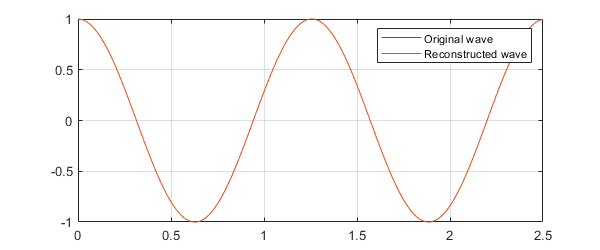
\includegraphics[height=3cm]{Figures/Signal/cos5x_100.png}
}%
\hspace*{\fill}
\subfloat[]{%
  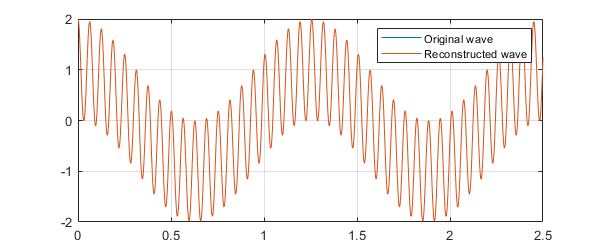
\includegraphics[height=3cm]{Figures/Signal/cos10x_cos20x_100.png}
}%
\\
\hspace*{\fill}
\subfloat[]{%
  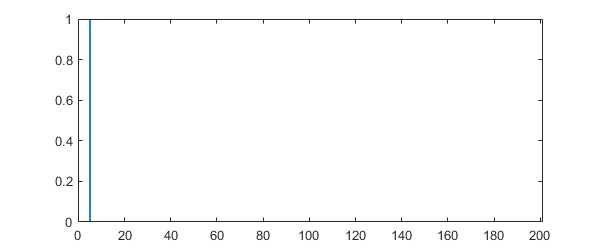
\includegraphics[height=3cm]{Figures/Signal/cos5x_100_bar.png}
}%
\hspace*{\fill}
\subfloat[]{%
  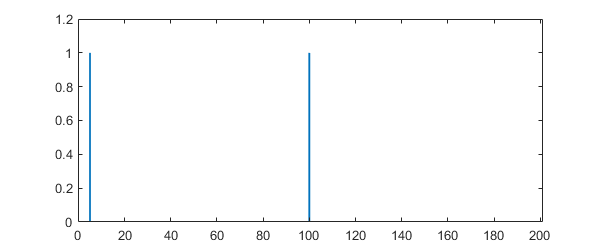
\includegraphics[height=3cm]{Figures/Signal/cos10x_cos20x_100_barplot.png}
}
\hspace*{\fill}
\caption{(\textbf{a}) Plot overlapping the original signal $f(x) = \cos(5x)$ used for sampling and the reconstructed sum of cosines approximation;
(\textbf{b}) Overlap plot for $f(x) = \cos(5x) + \cos(100x)$.
(\textbf{c,d}) Histogram visualizing the sparsity of the solution coefficients for both the solution vectors.}
\label{fig:cos_fitting}
\end{figure}

In Figure \ref{fig:cos_fitting}.c a single peak on the 5th component is noticeable, while in Figure \ref{fig:cos_fitting}.d two peaks emerge on the 5th and 100th component of the solution vector $x$ describing which sine frequency is involved in reconstructing the signal.

Further experimental results are provided for signals unexpressable using a finite sum of cosine or sine functions. We have used the square, triangle and sawtooth waves already presented in starting sections. The quality of the solution in terms of satisfying the constraints has been verified by computing the distance $\norm{Ax-b}_2$, which is under the machine epsilon for each of the ran experiments.


\begin{table}[htb]
    \centering
    \begin{tabular}{@{}cccccccc@{}}
        \toprule
        n & m & $\norm{Ax-b}_2$ & $\norm{x}_1$ & MSE & $\rho$ & t(s) & Iterations\\
        \midrule
        & &  & Square wave & \\
        \bottomrule
        \textbf{1000} & \textbf{500} & \boldmath{$6.184049\times 10^{-12}$} & \boldmath{$1.191508\times 10^{1}$} & \boldmath{$4.759236\times 10^{-2}$} & \textbf{0.994039} & 2.635641 & 1668 \\
        1000 & 200 & $1.336977\times 10^{-12}$ & $1.030814\times 10^{1}$ & $1.375599\times 10^{-1}$ & 0.983268 & 1.579137 & 747 \\
        1000 & 100 & $9.115071\times 10^{-13}$ & $8.962806$ & $5.639264\times 10^{-1}$ & 0.928024 & 0.703848 & 405\\
        \bottomrule
        & &  & Triangle wave & \\
        \bottomrule
        \textbf{1000} & \textbf{300} & \boldmath{$4.855598\times 10^{-12}$} & \boldmath{$2.785807$} &  \boldmath{$4.984034\times 10^{-5}$} & \textbf{0.999982} & 2.367487 & 917  \\
        1000 & 150 & $1.314703\times 10^{-13}$ & $2.758031$ & $3.348301\times 10^{-4}$ & 0.999890 & 1.172209 & 537  \\
        1000 &  50 & $3.862848\times 10^{-14}$ & $2.602165$ & $5.337773\times 10^{-3}$ & 0.998155 & 0.242113 & 183 \\
        \bottomrule
        & &  & Sawtooth wave & \\
        \bottomrule
         \textbf{1000} & \textbf{300} & \boldmath{$1.541872\times 10^{-12}$} & \textbf{9.820195} & \boldmath{$3.793370\times 10^{-2}$} & \textbf{0.985887} & 2.101900 & 972 \\
        1000 & 200 & $8.201787\times 10^{-13}$ & 8.326592 & $1.615636\times 10^{-1}$ & 0.938157 & 1.679192 & 712 \\
        1000 & 100 & $9.999465\times 10^{-14}$ & 5.401452 & $4.949854\times 10^{-1}$ & 0.797561 & 0.745310 & 409\\
    \end{tabular}
     \caption{Parameters and metrics for the sum of cosines reconstruction task, using trivial finite sums of cosines class of functions.}
     \label{table:sq_tr_saw}
\end{table}

The top results in terms of MSE and $\rho$, obtained by using the best trade-off amongst number of variables and number of observations can be visualized in Figure \ref{fig:square_tr_saw}. 

\begin{figure}[H]
\centering
\hspace*{\fill}
\subfloat[]{%
  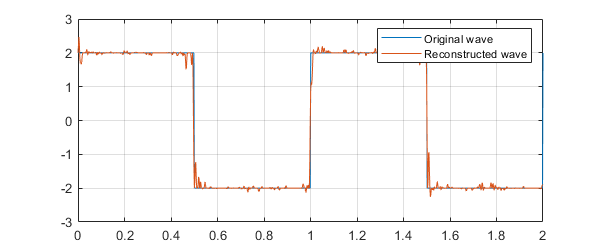
\includegraphics[height=3.5cm]{Figures/Signal/square500.png}
}%
\hspace*{\fill}
\subfloat[]{%
  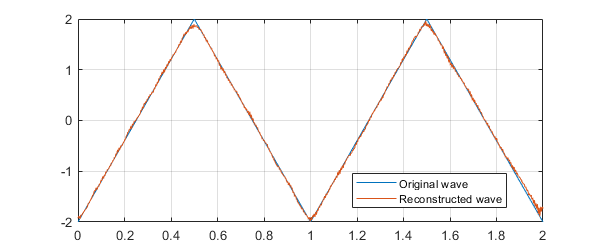
\includegraphics[height=3.5cm]{Figures/Signal/triangle500.png}
}%
\newline
\centering
\subfloat[]{%
  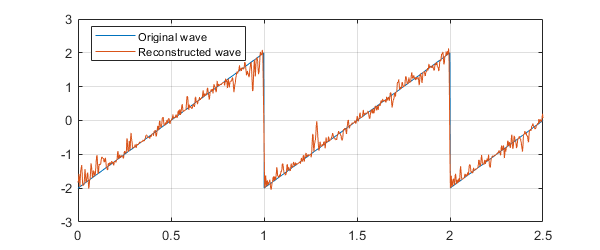
\includegraphics[height=3.5cm]{Figures/Signal/sawtooth300.png}
}%

\caption{Overlapping of the original signal in blue $f(x)$ used for sampling and the reconstructed sum of cosines approximation $\hat{f}(x)$,
(\textbf{a}) Square wave using n=1000 and m = 500,
(\textbf{b}) Triangle wave using n=1000 and m = 300,
(\textbf{c}) Sawtooth wave using n=1000 and m = 300.}
\label{fig:square_tr_saw}
\end{figure}

Despite the good results shown in Table \ref{table:sq_tr_saw}, from our approach, a comparison is a required step in order to assess the correctness and efficiency of the proposed solution. As from our previous knowledge on simplex which is a bound solver in linear programming will find the optimal result in much more longer time when compared with IPM solver from Matlab. Hence, the iterations are a bit longer but the requirements on the constraints and distance metrics are more precise.

The quicker algorithm ( Interior point method ) from table \ref{tab:IPM_res} results in having a lower number of iterations and could reach optimal condition by moving inside the feasible region trying to pass as many corners on the boundary. In the case of IPM, the iterations are relatively less than simplex methods as it is independent with the size of the problem.

When we compare both the approaches keenly, we observe the triangle wave and the sawtooth wave have been reasonably good for both dual and Interior point methods. However if the IPM is faster, the dual simplex results for MSE and $\rho$ are far better.


%TODO{Search on differences (literature) between IPM and dual -> Write something here citing the results on the table from Appendix A1}


\subsection{ECG reconstruction}

The results for the second application cover different ECG signals sampled at 0.7 kHz for 3 seconds ranging from 3 different set of heart-beating conditions:

\begin{itemize}
    \item Bradycardia: signals lower than 60 BPM
    \item Tachycardia: signals above 100 BPM
    \item Sinus rhythm: remaining average signals
\end{itemize}

Each signal utilized in this section have been generated by a Matlab Toolbox for ECG simulation, updating the original code in order to accept different parameters such as timing, frequency, and beats per minute (BPM).
The objective of this specific application is that of reconstructing an original signal sampled at a certain frequency over time, considering partial observations according to a pre-defined Compression Ratio (CR).

In Figure \ref{fig:bradycardia}, we provide the resulting overlap amongst the reconstructed and a signal sampled at 0.7kHz for 3 seconds having 40BPM with two different CR (90\% on the left, 80\% on the right). The result obtained by using 90\% CR, appears noisy and needs more observations, also due to the nature of the signal having a low number of characterizing peaks. Instead, the signal in Figure \ref{fig:bradycardia}.b, by utilizing 20\% of the original wave gets a reconstruction without visually appreciable differences.

\begin{figure}[H]
\centering
\hspace*{\fill}
\subfloat[]{%
  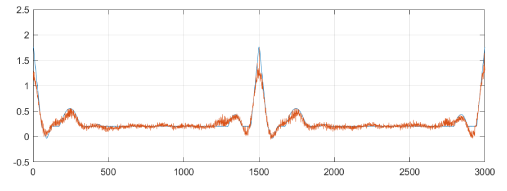
\includegraphics[height=3cm]{Figures/ECG/BPM40_CR90edit.png}
}%
\hspace*{\fill}
\subfloat[]{%
  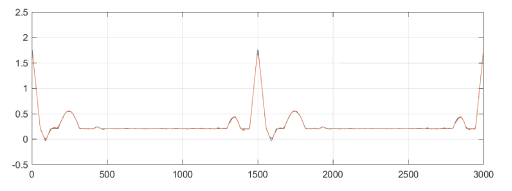
\includegraphics[height=3cm]{Figures/ECG/BPM40_CR80edit.png}
}%
\hspace*{\fill}
\caption{ECG signal sampled at 0.7kHz for 3 seconds having an average of 40 beats per minute showing bradycardia, (\textbf{a}) Overlapping the original and the reconstructed signal using 80\% CR. 
(\textbf{b}) Overlapping the original and the reconstructed signal using 90\% CR.}
\label{fig:bradycardia}
\end{figure}

By using the same procedure, in Figure \ref{fig:sinus}, we show a different signal having around 60BPM. Apparently, each signal belonging to this class show good results even by using only 10\% of the original observation. We should also mention that, the sparsity assumption for compressive sensing is guaranteed by applying DCT to the signal as shown in introductory sections.

\begin{figure}[H]
\centering
\hspace*{\fill}
\subfloat[]{%
  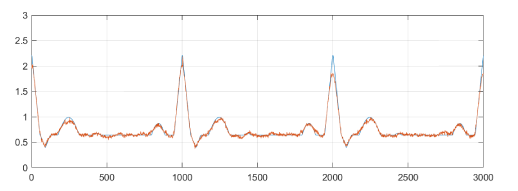
\includegraphics[height=3cm]{Figures/ECG/BPM60_CR90edit.png}
}%
\hspace*{\fill}
\subfloat[]{%
  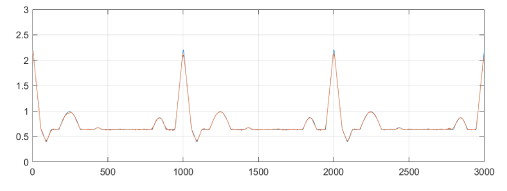
\includegraphics[height=3cm]{Figures/ECG/BPM60_CR80edit.png}
}%
\hspace*{\fill}
\caption{ECG signal sampled at 0.7kHz for 3 seconds having an average of 60 beats per minute having sinus rhythm, (\textbf{a}) Overlapping the original and the reconstructed signal using 80\% CR. 
(\textbf{b}) Overlapping the original and the reconstructed signal using 90\% CR.}
\label{fig:sinus}
\end{figure}

Lastly we analyze a signal sampled at the same frequency rate, but having 120BPM. The high number of peaks plays a huge role in identifying a good reconstruction even by using 80\% CR. In Figure \ref{fig:tachycardia} we can appreciate the overall good qualitative quality of each of the two experiments.

\begin{figure}[H]
\centering
\hspace*{\fill}
\subfloat[]{%
  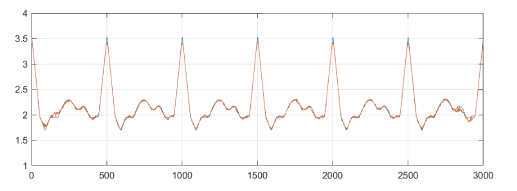
\includegraphics[height=3cm]{Figures/ECG/BPM120_CR90edit.png}
}%
\hspace*{\fill}
\subfloat[]{%
  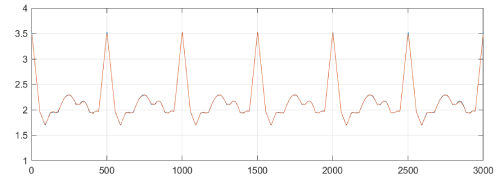
\includegraphics[height=3cm]{Figures/ECG/BPM120_CR80edit.png}
}%
\hspace*{\fill}
\caption{ECG signal sampled at 0.7kHz for 3 seconds having an average of 120 beats per minute showing tachycardia, (\textbf{a}) Overlapping the original and the reconstructed signal using 80\% CR. 
(\textbf{b}) Overlapping the original and the reconstructed signal using 90\% CR.}
\label{fig:tachycardia}
\end{figure}

As we did previously for different waves we provide an extensive table showing a subset with the most meaningful experiments ran by measuring MSE and correlation coefficient amongst the original and the reconstructed one by using a specific compression ratio (Table \ref{table:ecg}). Expectedly by decreasing the compression ratio which is involved in increasing the number of observations 'm', the quality of the reconstruction increases as a result. The solutions found appear to be adequately sparse according to the L-1 norm of the solution vector which is always at least one order of magnitude smaller than the original number of variables 'n'.

The notations $x$ and $x^*$ stand respectively for the original DCT vector and the solution obtained by the dual. In order to ensure correctness of the objective value we compared the accuracy of our optimal value compared to the target, and computing the distance $\norm {x^* - x}_2$, reported in the second last column of Table \ref{table:ecg}. A visual representation of both the vectors is shown in the second column of the first and second rows in Figure \ref{fig:ecg_appendix}.


\begin{table}[htb]
    \centering
    \begin{tabular}{@{}llllllll@{}}
        \toprule
        BPM & n & m & \norm{x^*}_1 & MSE & $\rho$ & \norm{x^* - x}_2 & CR \\
        \midrule
        40 & 2100 & 750 &  92.456816 & $7.0 \times 10^{-6}$ & 0.999947 &
        0.249430 & 75\%  \\
        40 & 2100 & 600 &  91.442043 & $1.09 \times 10^{-4}$ & 0.999247 & 0.252230 & 80\%  \\
        40 & 2100 & 300 &  82.738883 & $3.905 \times 10^{-3}$ & 0.975843 & 0.234737 & 90\%  \\
        120 & 2100 & 750 &  190.433072 & $8.0 \times 10^{-6}$ & 0.999975 & 9.456573 & 75\%  \\
        120 & 2100 & 600 &  189.810936 & $4.8 \times 10^{-5}$ & 0.999841 & 9.458531 & 80\%  \\
        120 & 2100 & 300 &  185.153483 & $7.24 \times 10^{-4}$ & 0.997722 & 9.435898 & 90\% \\
        70 & 2100 & 750 &  120.201399 & $4.8 \times 10^{-5}$ & 0.999760 & 2.089961 & 75\% \\
        70 & 2100 & 600 &   119.479618 & $1.36 \times 10^{-4}$ & 0.999354 & 2.088543 & 80\%  \\
        70 & 2100 & 300 & 114.867033 & $2.203 \times 10^{-3}$ & 0.990945 & 2.080364 & 90\% \\
        \bottomrule
    \end{tabular}
    \caption{Different signals have been sampled at 0.7kHz for 3 seconds describing different heart-beating conditions (40, 60, 90 BPM) and different compression rates (75\%, 80\%, 90\%). We reported the dimensions of the problem as long as the objective function value and two different distances for signals: Mean Squared Error (MSE) and correlation coefficient ($\rho$).}
    \label{table:ecg}
\end{table}

\clearpage
\subsection{Forrest Tomlin experiments}

The naive approach for revised dual simplex method initially performs a matrix inversion and subsequently solves three systems for each iteration. The latter has an approximate cost of $O(n^3)$ for the matrix inversion and three times $O(n^3)$ for the systems to be solved.

Several approaches exist for exploiting a persistent rank-1 update of a matrix over several iterations. Specifically, the FT update relies on computing a new LU factorization once in a while (according to the number of iterations considered for matrix refactor) having an approximate cost of $O(n^3)$. Now, the three different systems can be easily solved with the LU updated representation by having a reduced approximate cost of $O(n^2)$ times three.

In Figure \ref{fig:ft} we provide a graphical representation of the time of convergence for a single test iteration considering both the standard inverse approach and the FT. Along the y-axis we reported the average time for each iteration and on the x-axis the growing factor \emph{'m'}, representing matrix size. As we can see from the plot, there is an average improvement of one order of magnitude for the second approach over the first which suggests his suitability for the method. Further investigations can be run for assessing matrix stability and other useful properties for an LP solver.

\begin{figure}[H]
\centering
\subfloat{
  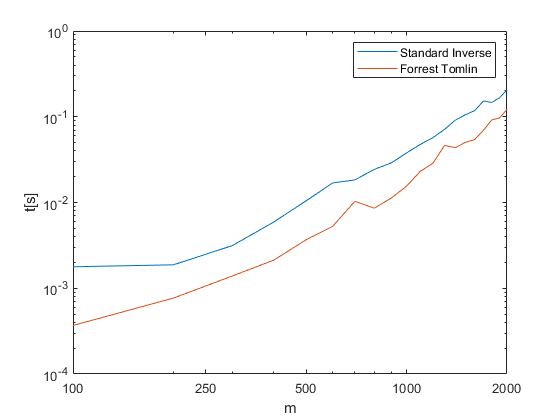
\includegraphics[height=6cm]{Figures/ECG/tom.png}
}
\caption{ Single iteration time of convergence line chart for the standard inverse approach in revised dual simplex and undergoing a FT update procedure. The Y-axis represents the time elapsed in seconds on a logarithmic scale and the x-axis grows in terms of matrix size.}
\label{fig:ft}
\end{figure}



\clearpage

\appendixtitles{no} %Leave argument "no" if all appendix headings stay EMPTY (then no dot is printed after "Appendix A"). If the appendix sections contain a heading then change the argument to "yes".
\appendix
\section{}
\begin{table}[htb]
    \centering
    \caption{Parameters and metrics for the sum of cosines reconstruction task using Interior Point Method from Matlab.}
    \begin{tabular}{@{}cccccccc@{}}
        \toprule
        n & m & $\norm{Ax-b}_2$ & $\norm{x}_1$ & MSE & $\rho$ & t(s) & Iterations \\
        \midrule
        & &  & Square wave & & \\
        \bottomrule
        1000 & 500 & 3.050674e-13 & 3.341861e+01 & 1.108982e+00 & 0.862073 & 0.235785 & 13 \\
        1000 & 300 & 1.150347e-08 & 1.832515e+01 & 7.908519e-01 & 0.895906 & 0.073733 & 15 \\
        1000 & 200 & 1.476637e-13 & 1.545430e+01 & 7.378967e-01 & 0.903961 & 0.053216 & 13 \\
        1000 & 100 & 3.882353e-14 & 1.120629e+01 & 1.750944e+00 & 0.750045 & 0.023976 & 12 \\
        \bottomrule
        & &  & Triangle wave & \\
        \bottomrule
        1000 & 300 & 2.764943e-10 & 6.319097e+00 & 9.239564e-02 & 0.964813 & 0.069409 & 13 \\
        1000 & 150 & 2.290984e-11 & 4.211512e+00 & 8.833424e-02 & 0.966517 & 0.031550 & 13 \\
        1000 &  50 & 1.364053e-11 & 2.986549e+00 & 1.121243e-01 & 0.959723 & 0.007290 & 11 \\
        \bottomrule
        & &  & Sawtooth wave & \\
        \bottomrule
        1000 & 300 & 1.037120e-11 & 1.217783e+01 & 4.255144e-01 & 0.826686 & 0.076458 & 13 \\
        1000 & 200 & 1.215180e-11 & 1.100427e+01 & 6.029744e-01 & 0.746856 & 0.053002 & 12 \\
        1000 & 100 & 3.162498e-12 & 6.582426e+00 & 8.374424e-01 & 0.614149 & 0.022410 & 12 \\
        \bottomrule
    \end{tabular}
    \label{tab:IPM_res}
\end{table}

\begin{figure}[H]
\centering
\subfloat{
  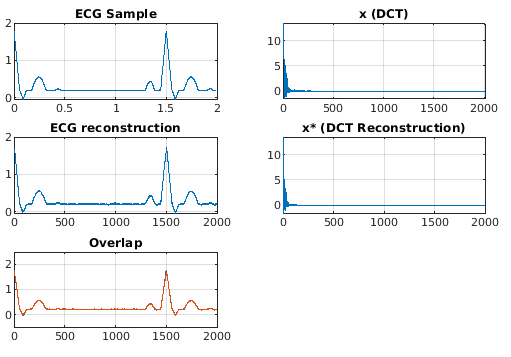
\includegraphics[height=8cm]{Figures/ECG/rec.png}
}
\caption{ECG signal sampled at 1kHz for 2 seconds having an average of 60 beats per minute. The overall pipeline is depicted here in a top-down sequence, the signal undergoes sampling and discrete cosine transform obtaining the original vector x. After solving the optimization system we retrieve $x^*$ from which we performIDCT and  }
\label{fig:ecg_appendix}
\end{figure}

\begin{figure}[H]
\centering
\hspace*{\fill}
\subfloat[]{%
  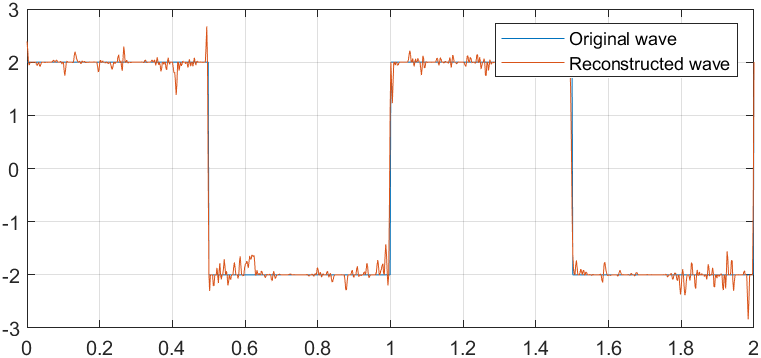
\includegraphics[height=3.5cm]{Figures/square.png}
}%
\hspace*{\fill}
\subfloat[]{%
  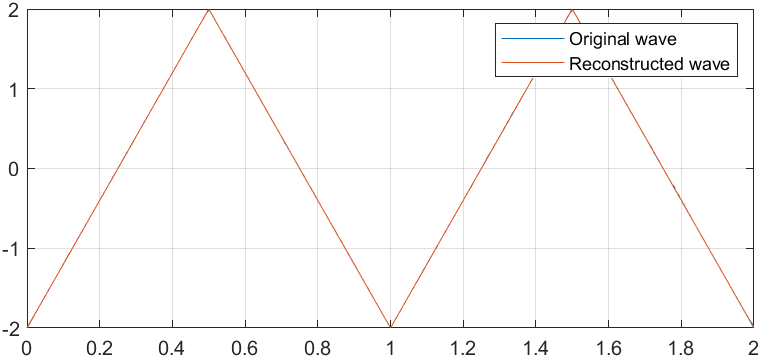
\includegraphics[height=3.5cm]{Figures/triangle.png}
}%
\newline
\centering
\subfloat[]{%
  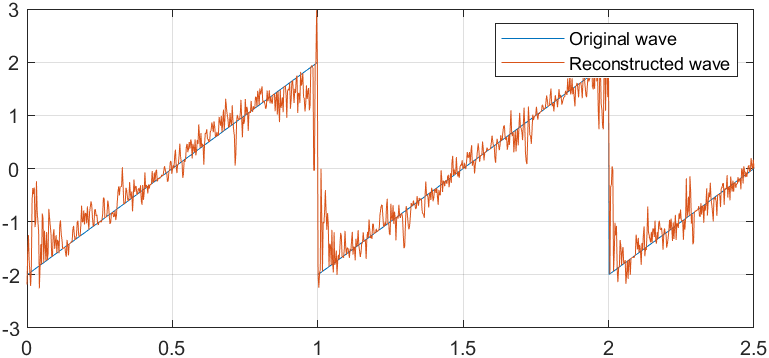
\includegraphics[height=3.5cm]{Figures/sawtooth.png}
}%

\caption{IPM method solutions overlapping of the original signal in blue $f(x)$ used for sampling and the reconstructed sum of cosines approximation $\hat{f}(x)$,
(\textbf{a}) Square wave using n=1000 and m = 500,
(\textbf{b}) Triangle wave using n=1000 and m = 300,
(\textbf{c}) Sawtooth wave using n=1000 and m = 300.}
\label{fig:IPM_square_sawtooth_tr}
\end{figure}

\reftitle{References}
\externalbibliography{yes}
\bibliography{bibliography}
\end{document}

